\documentclass[usenames,dvipsnames]{beamer}

\mode<presentation> {
\usetheme{Montpellier}
}

\usepackage{graphicx} % Allows including images
\usepackage{booktabs} % Allows the use of \toprule, \midrule and \bottomrule in tables
\usepackage[frenchb]{babel}
\usepackage[T1]{fontenc}
\usepackage[utf8]{inputenc}
\usepackage{algorithm2e}
\setcounter{tocdepth}{2}
\graphicspath{{../../Figures/}}


\DeclareMathOperator*{\argmin}{arg\,min}
\DeclareMathOperator*{\argmax}{arg\,max}
\newtheorem*{proposition}{Proposition}
\newcommand\Fontvi{\fontsize{8}{8}\selectfont}

% exercices comptés
\newcounter{numexos}%Création d'un compteur qui s'appelle numexos
\setcounter{numexos}{0}%initialisation du compteur
\newcommand{\exercice}[1]{%Création d'une macro ayant un paramètre
\addtocounter{numexos}{1}%chaque fois que cette macro est appelée, elle ajoute 1 au compteur numexos
\textcolor{DarkOrchid}{Exercice\,\thenumexos\,:}\,#1%Met en rouge Exercice et la valeur du compteur appelée par \thenumeexos
}

\setbeamertemplate{title page}{
    \centering

    \Large\bfseries
    Machine learning Tek 5: classification and regression trees

\begin{figure}[!h]
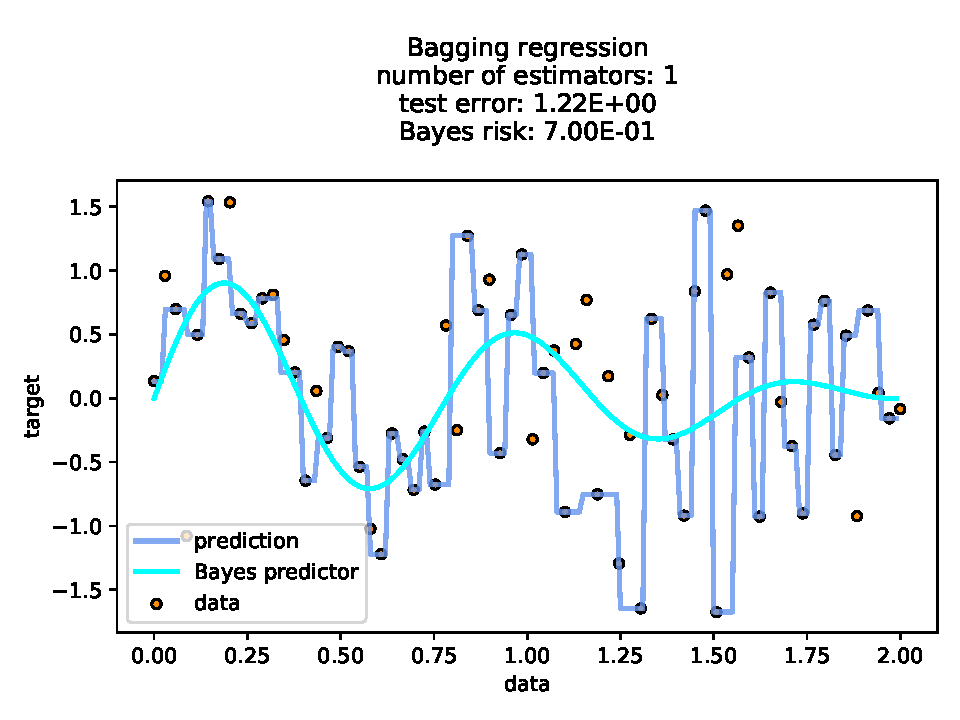
\includegraphics[width=8cm]{bagging/Bagging_regression_nest_1}
\end{figure}

    }

\title[FTML]{title}


\date{} % Date, can be changed to a custom date

\makeatletter
\let\@@magyar@captionfix\relax
\makeatother

\begin{document}

\begin{frame}
\titlepage % Print the title page as the first slide
\end{frame}

\section*{Introduction} % (fold)
\label{sec:section_name}

\begin{frame}
\frametitle{} % Table of contents slide, comment this block out to remove it
\tableofcontents % Throughout your presentation, if you choose to use \section{} and \subsection{} commands, these will automatically be printed on this slide as an overview of your presentation
\end{frame}

\section{Decision trees}%
\label{sec:decision_trees}

\subsection{Decision trees}%
\label{sub:decision_trees}

\begin{frame}{Example dataset: fishes}
    \begin{figure}[htpb]
        \centering
        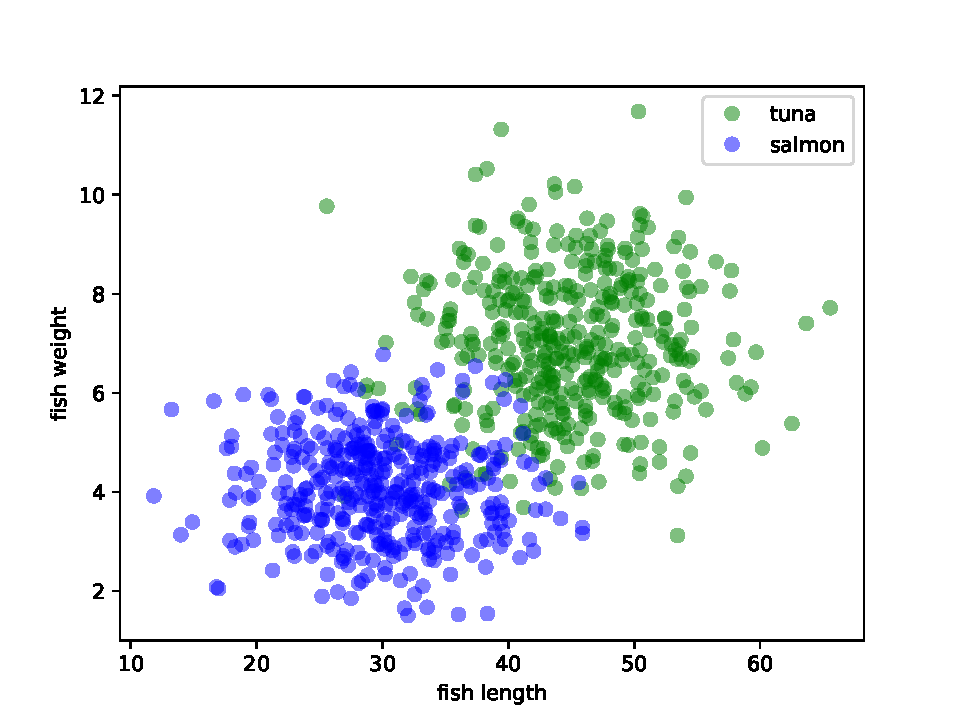
\includegraphics[width=0.8\linewidth]{fish_scatter_plot}
        \label{fig:fish_scatter_plot}
    \end{figure}
\end{frame}

\begin{frame}{Fish dataset}
    \begin{figure}[htpb]
        \centering
        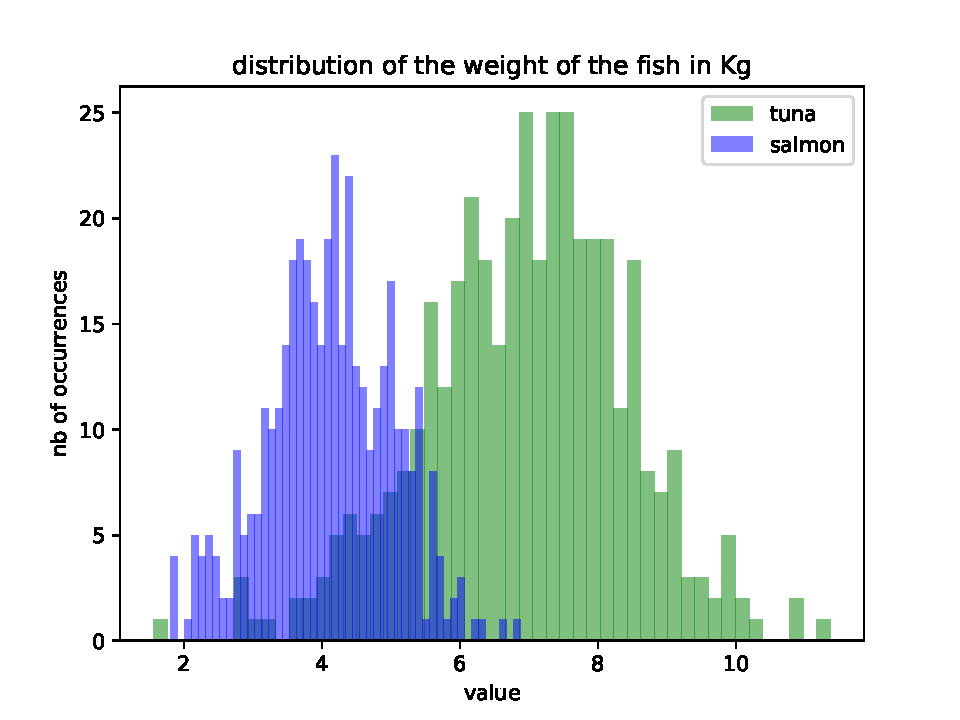
\includegraphics[width=0.8\linewidth]{fish_weight_with_class}
        \label{fig:fish_weight_with_class}
    \end{figure}
\end{frame}


\begin{frame}{Fish dataset}
    \begin{figure}[htpb]
        \centering
        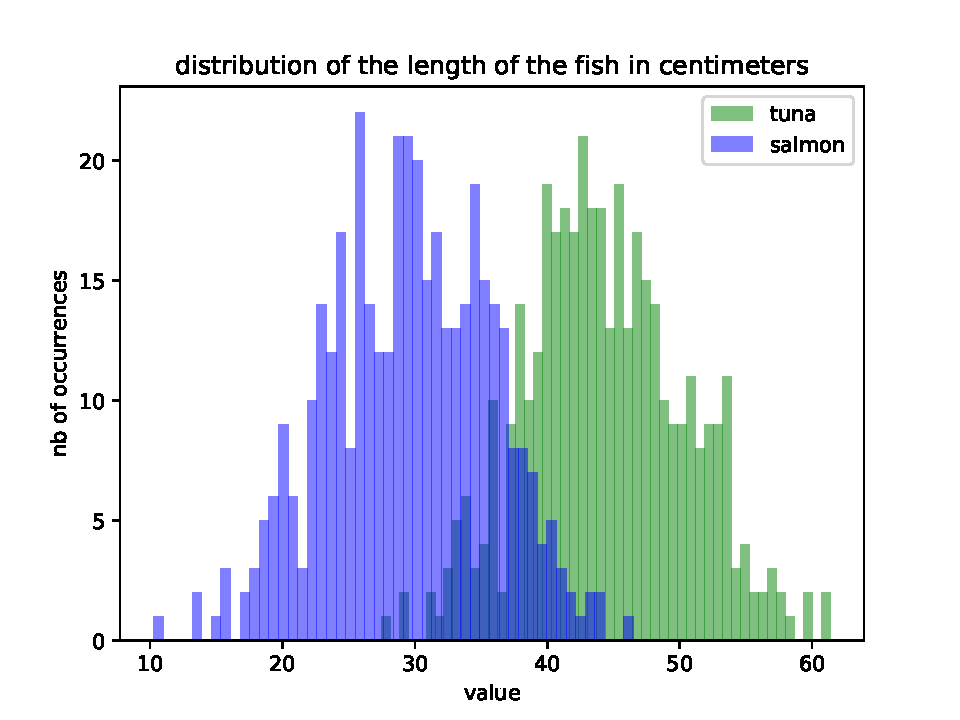
\includegraphics[width=0.8\linewidth]{fish_length_with_class}
        \label{fig:fish_weight_with_class}
    \end{figure}
\end{frame}

\begin{frame}{CART}
    \begin{itemize}
	\item Segmentation method (partitionnement récursif), \textbf{{binary splits.}} 
	\item First algorithm: \textbf{{CART}} (classification and regression tree, Breiman, 1984) \cite{Breiman2017} 
    \end{itemize}
\end{frame}



\begin{frame}{Example tree}
    \begin{figure}[htpb]
	\centering
	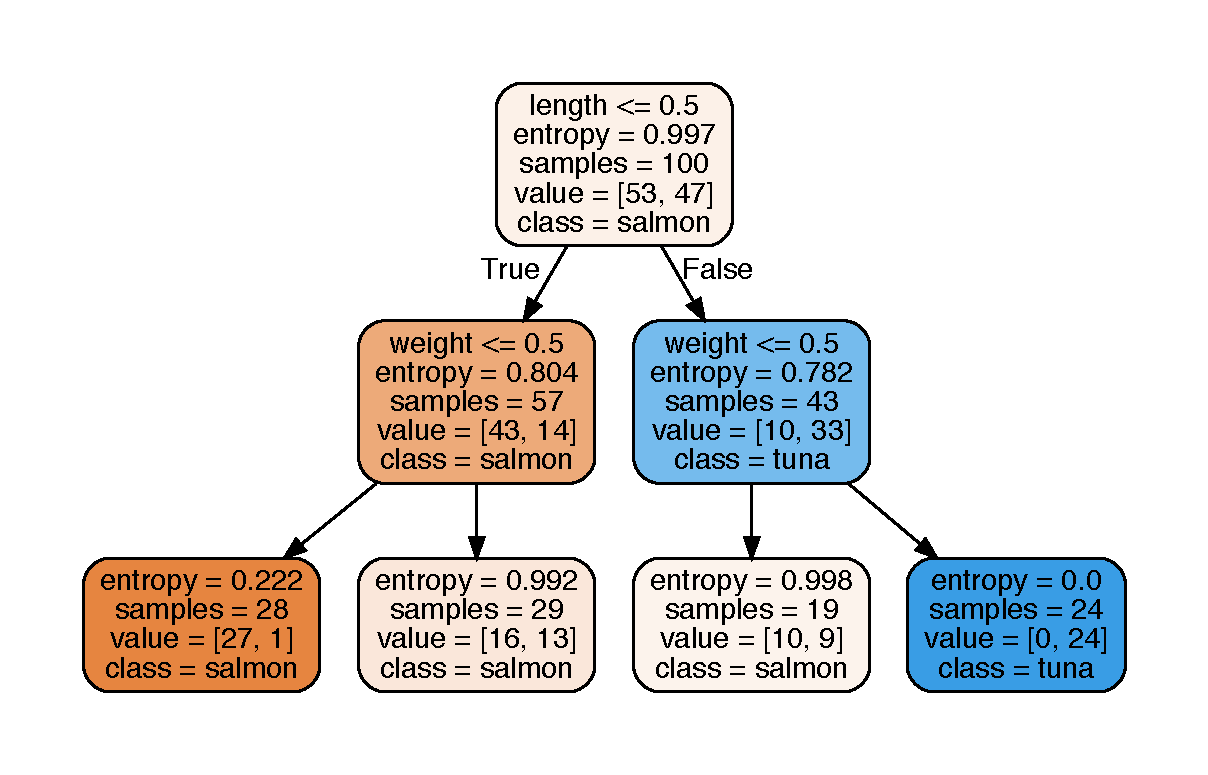
\includegraphics[width=0.75\linewidth]{fish_minimal_max_depth_2}
	\label{fig:name}
    \end{figure}
    Each split should lead to more \textbf{{homogeneous}} nodes (in a sense that is to be formally defined)
\end{frame}

\begin{frame}{Leaves}
    Leaf nodes correspond to a predicted value (class or real number for instance if $ \mathcal{Y}  = \mathbb{R} )$).

    \begin{figure}[htpb]
	\centering
	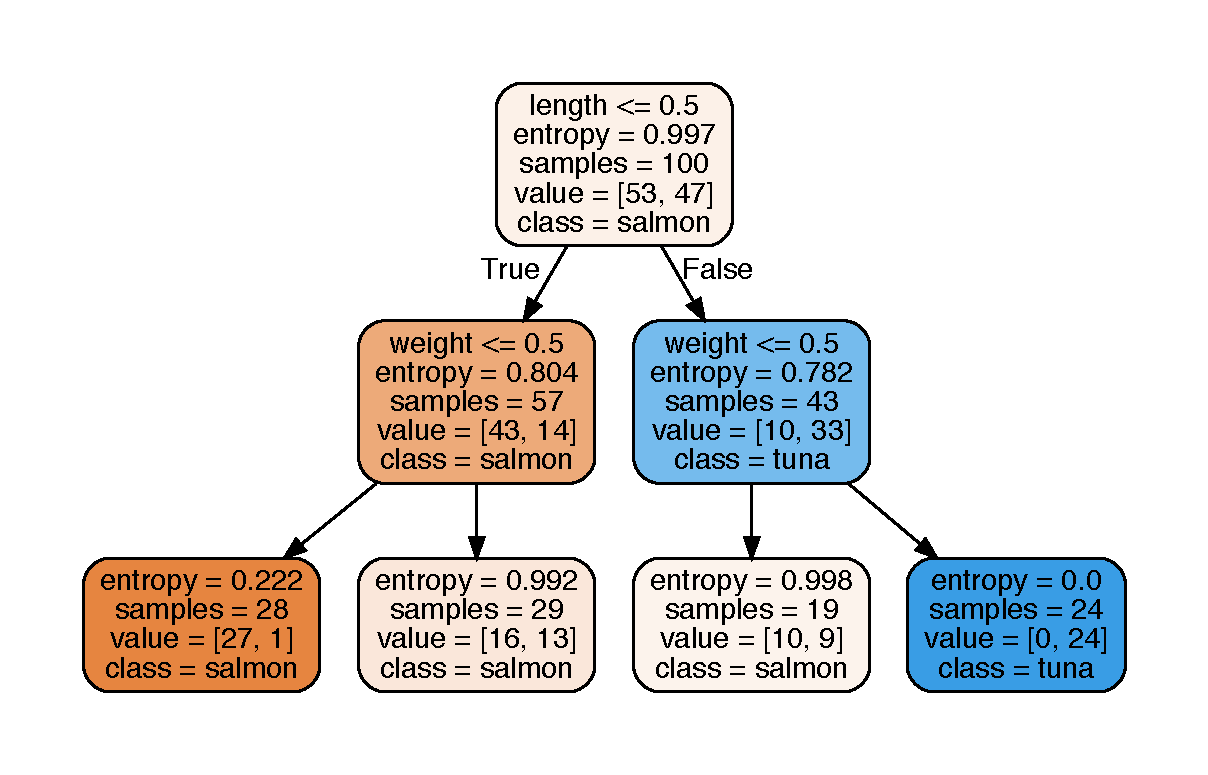
\includegraphics[width=0.75\linewidth]{fish_minimal_max_depth_2}
	\label{fig:name}
    \end{figure}
\end{frame}

\begin{frame}
    Decision trees can also be used for regression. In that case, the prediction is \textbf{{piecewise constant}}. It can be seen as a form of local averaging.

 \begin{figure}[htpb]
     \centering
     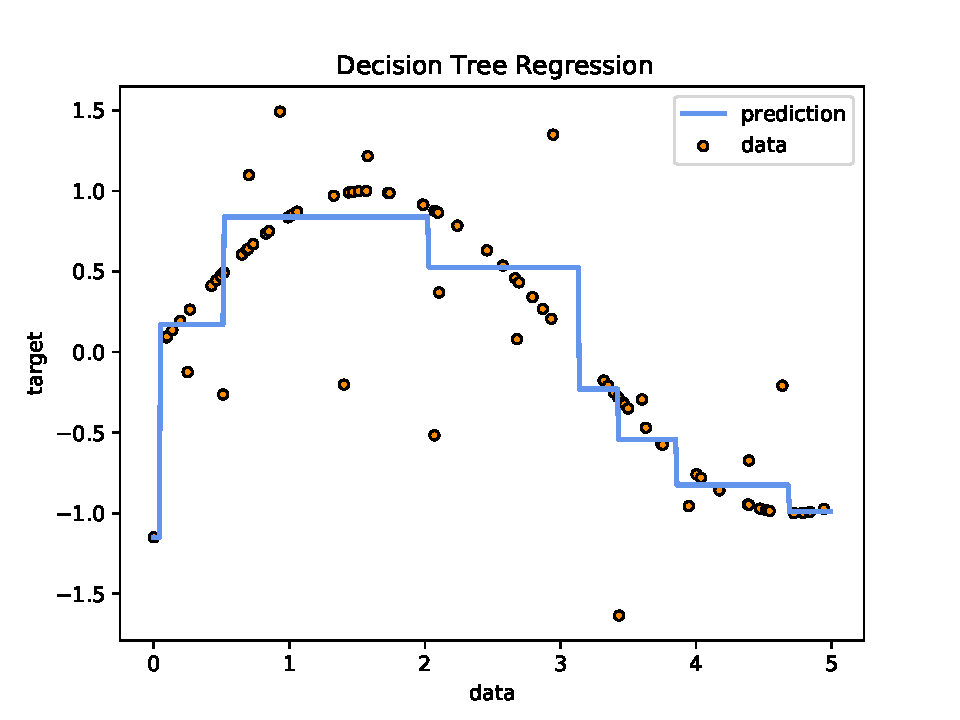
\includegraphics[width=0.7\linewidth]{decision_tree_regression}
     \label{fig:decision tree regression}
 \end{figure}
\end{frame}

\subsection{Construction of a decision tree}%
\label{sub:construction_of_a_decision_tree}

\begin{frame}{Construction of a tree}
    
    A split node corresponds to:
    \begin{itemize}
        \item a segmentation variable $V$
	\item a segmentation value / threshold if $V$ is quantitative. If $V$ is a class, it is a two-fold partitionning of the set of classes.
    \end{itemize}
   The construction of a tree requires a criterion to:
    \begin{itemize}
        \item choose the segmentation variable and value
	\item decide when a node is terminal (leaf node)
	\item associate a prediction value to all leaf nodes
    \end{itemize}
\end{frame}

\subsubsection{Segmentation criterion}
\label{ssub:segmentation_criterion}

\begin{frame}{Homogeneity}

    We want the homogeneity in the child nodes to be greater than in the parent node. Equivalently, we can define a non-negative heterogeneity function $H$ that describes each node and that must be:
    \begin{itemize}
	\item $0$ if the node is homogeneous (only one class (classification) or one output value (regression) is represented in this node).
	\item maximal if the values of $y$ are uniformly distributed within the node.
	\item if $H(L)$ it the value of $H$ for the left child node (and $H(R)$ for the right one), then the segmentation should minimize
	    \begin{equation}
		H(L)+H(R)
	    \end{equation}
    \end{itemize}
\end{frame}

\subsubsection{Homogeneity/heterogeneity criterion}%
\label{ssub:homogeneity_criterion}

\begin{frame}{Homogeneity criterion for regression}

    In the case of regression, $ \mathcal{Y}  = \mathbb{R} $ and the heterogeneity $H(n)$ of node $n$ is its empirical variance:
    \begin{equation}
	H(n) = \frac{1}{|n|} \sum_{i\in n} (y_i - \bar{y_n})^2
    \end{equation}

    Each $y_i$ is a label for an input $x_i$ that arrives in node $n$.
    
\end{frame}

\begin{frame}{Homogeneity criterion for classification}
    In the case of classification, $ \mathcal{Y}  = [1, \dots, L]$ and several criteria exist.  
\end{frame}

\begin{frame}{Homogeneity criterion for classification: entropy (information gain)}
    \begin{itemize}
        \item We use the convention that $ 0 \log (0) = 0$
	\item $p_n^l$ is the proportion of class $ l$ in node $n$.
    \end{itemize}
    The \textbf{{entropy}} writes:

    \begin{equation}
	H(n) = - \sum^{L}_{l=1} p_n^l\log( p_n^l)
    \end{equation}

    \exercice{\textbf{}}What are the maximum and minimum values of the entropy ?
\end{frame}

\begin{frame}{Homogeneity criterion for classification: Gini impurity}
    The Gini impurity writes:

    \begin{equation}
	H(n) = \sum^{L}_{l=1} p_n^l(1-p_n^l)
    \end{equation}
\end{frame}

\begin{frame}{Homogeneity criterion for classification: misclassification probability}
    \begin{equation}
	H(n) = 1-  \max_l(p_n^l)
    \end{equation}
    If we predict the most represented class in $n$, then this is the misclassification probability (if we assume that the classes are indeed distributed according to the proportions).
\end{frame}

\begin{frame}{Homogeneity criterion for classification: Gini impurity}
    \begin{equation}
	H(n) = \sum^{L}_{l=1} p_n^l(1-p_n^l)
    \end{equation}
    Same interpretation as the previous slide (misclassification probablity), but in the case we predict the classes according to the proportions in the leaves (instead of predicting the most likely class).
\end{frame}

\subsubsection{Prediction}%
\label{ssub:prediction}

\begin{frame}{Prediction for a leaf node}
    \begin{itemize}
        \item \textbf{{regression}}: predict the average value in the node
	\item \textbf{{classification}}: several possibilities
	    \begin{itemize}
	        \item most represented class in the node
		\item most probable class \textit{{a posteriori}} if the \textit{{a priori}} probabilities are known (Bayesian probabilities) 
		\item class that costs the less in case of missclassification
	    \end{itemize}
    \end{itemize}
\end{frame}


\subsection{Tree pruning}%
\label{sub:pruning}

\begin{frame}{Pruning}
    \begin{itemize}
	\item If the segmentation is not restricted, the tree can fit the training dataset perfectly (overfitting).
        \item learning would then be highly dependent on the choice of the training dataset, leading to \textbf{{instability.}} 
	\item To avoid it, \textbf{{pruning}} (élaguage) is used: it consists in restricting the size of the tree (and can be seen as an equivalent to regularization when we perform ridge regression of logistic regression). 
    \end{itemize}
\end{frame}

\begin{frame}{Pre-pruning by restricting divisions}
    We can impose
    \begin{itemize}
        \item minimum impurity decrease
        \item a minimum number of samples in a leaf node
        \item a minimum number of samples to authorize splitting a node
    \end{itemize}
\end{frame}

\begin{frame}{Simulation: fish dataset, max depth=1}
   \begin{figure}[htpb]
       \centering
       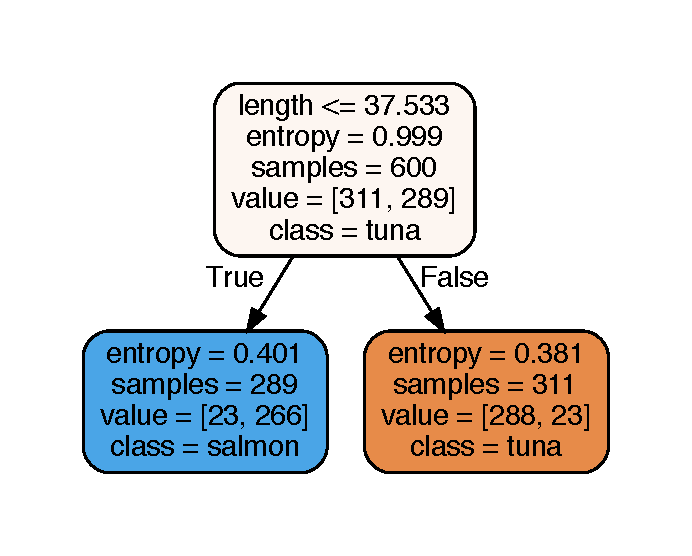
\includegraphics[width=0.7\linewidth]{fish_max_depth_1}
       \label{fig:}
   \end{figure} 
\end{frame}

\begin{frame}{Simulation: fish dataset}
   \begin{figure}[htpb]
       \centering
       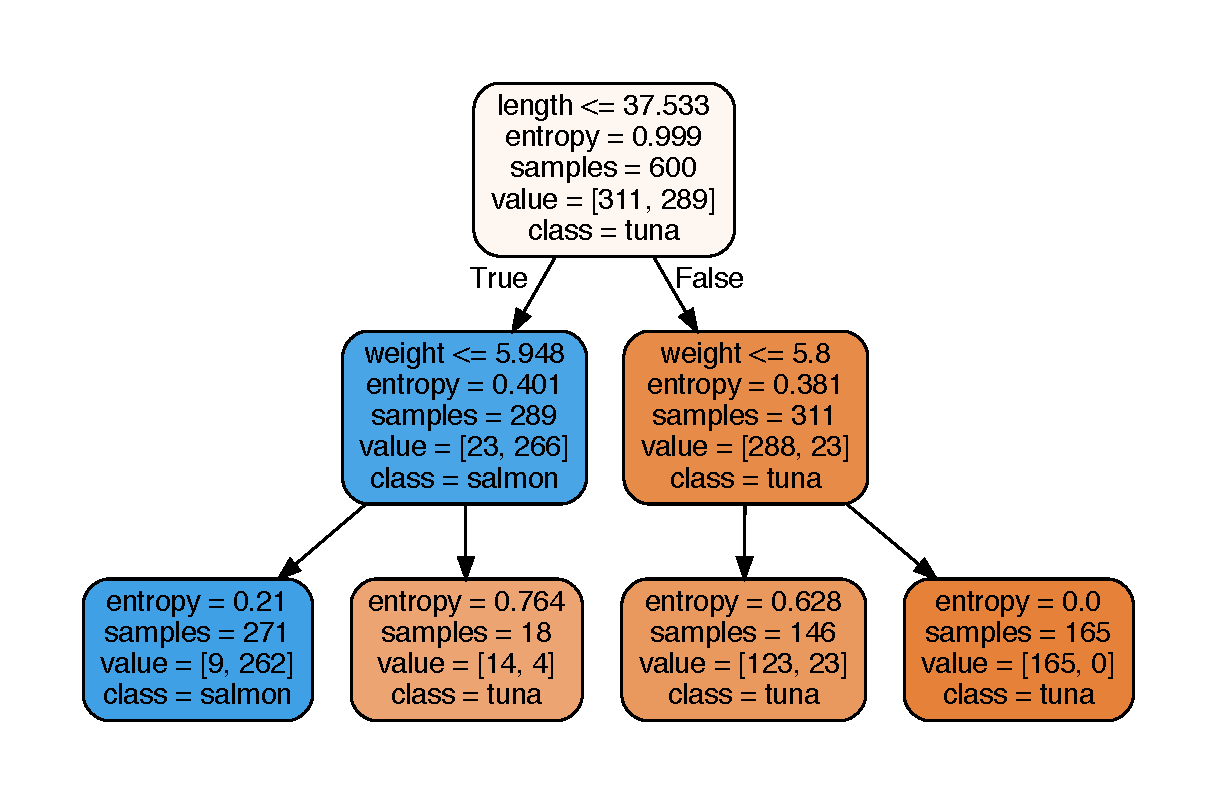
\includegraphics[width=0.7\linewidth]{fish_max_depth_2}
       \label{fig:}
   \end{figure} 
\end{frame}

\begin{frame}{Simulation: fish dataset}
   \begin{figure}[htpb]
       \centering
       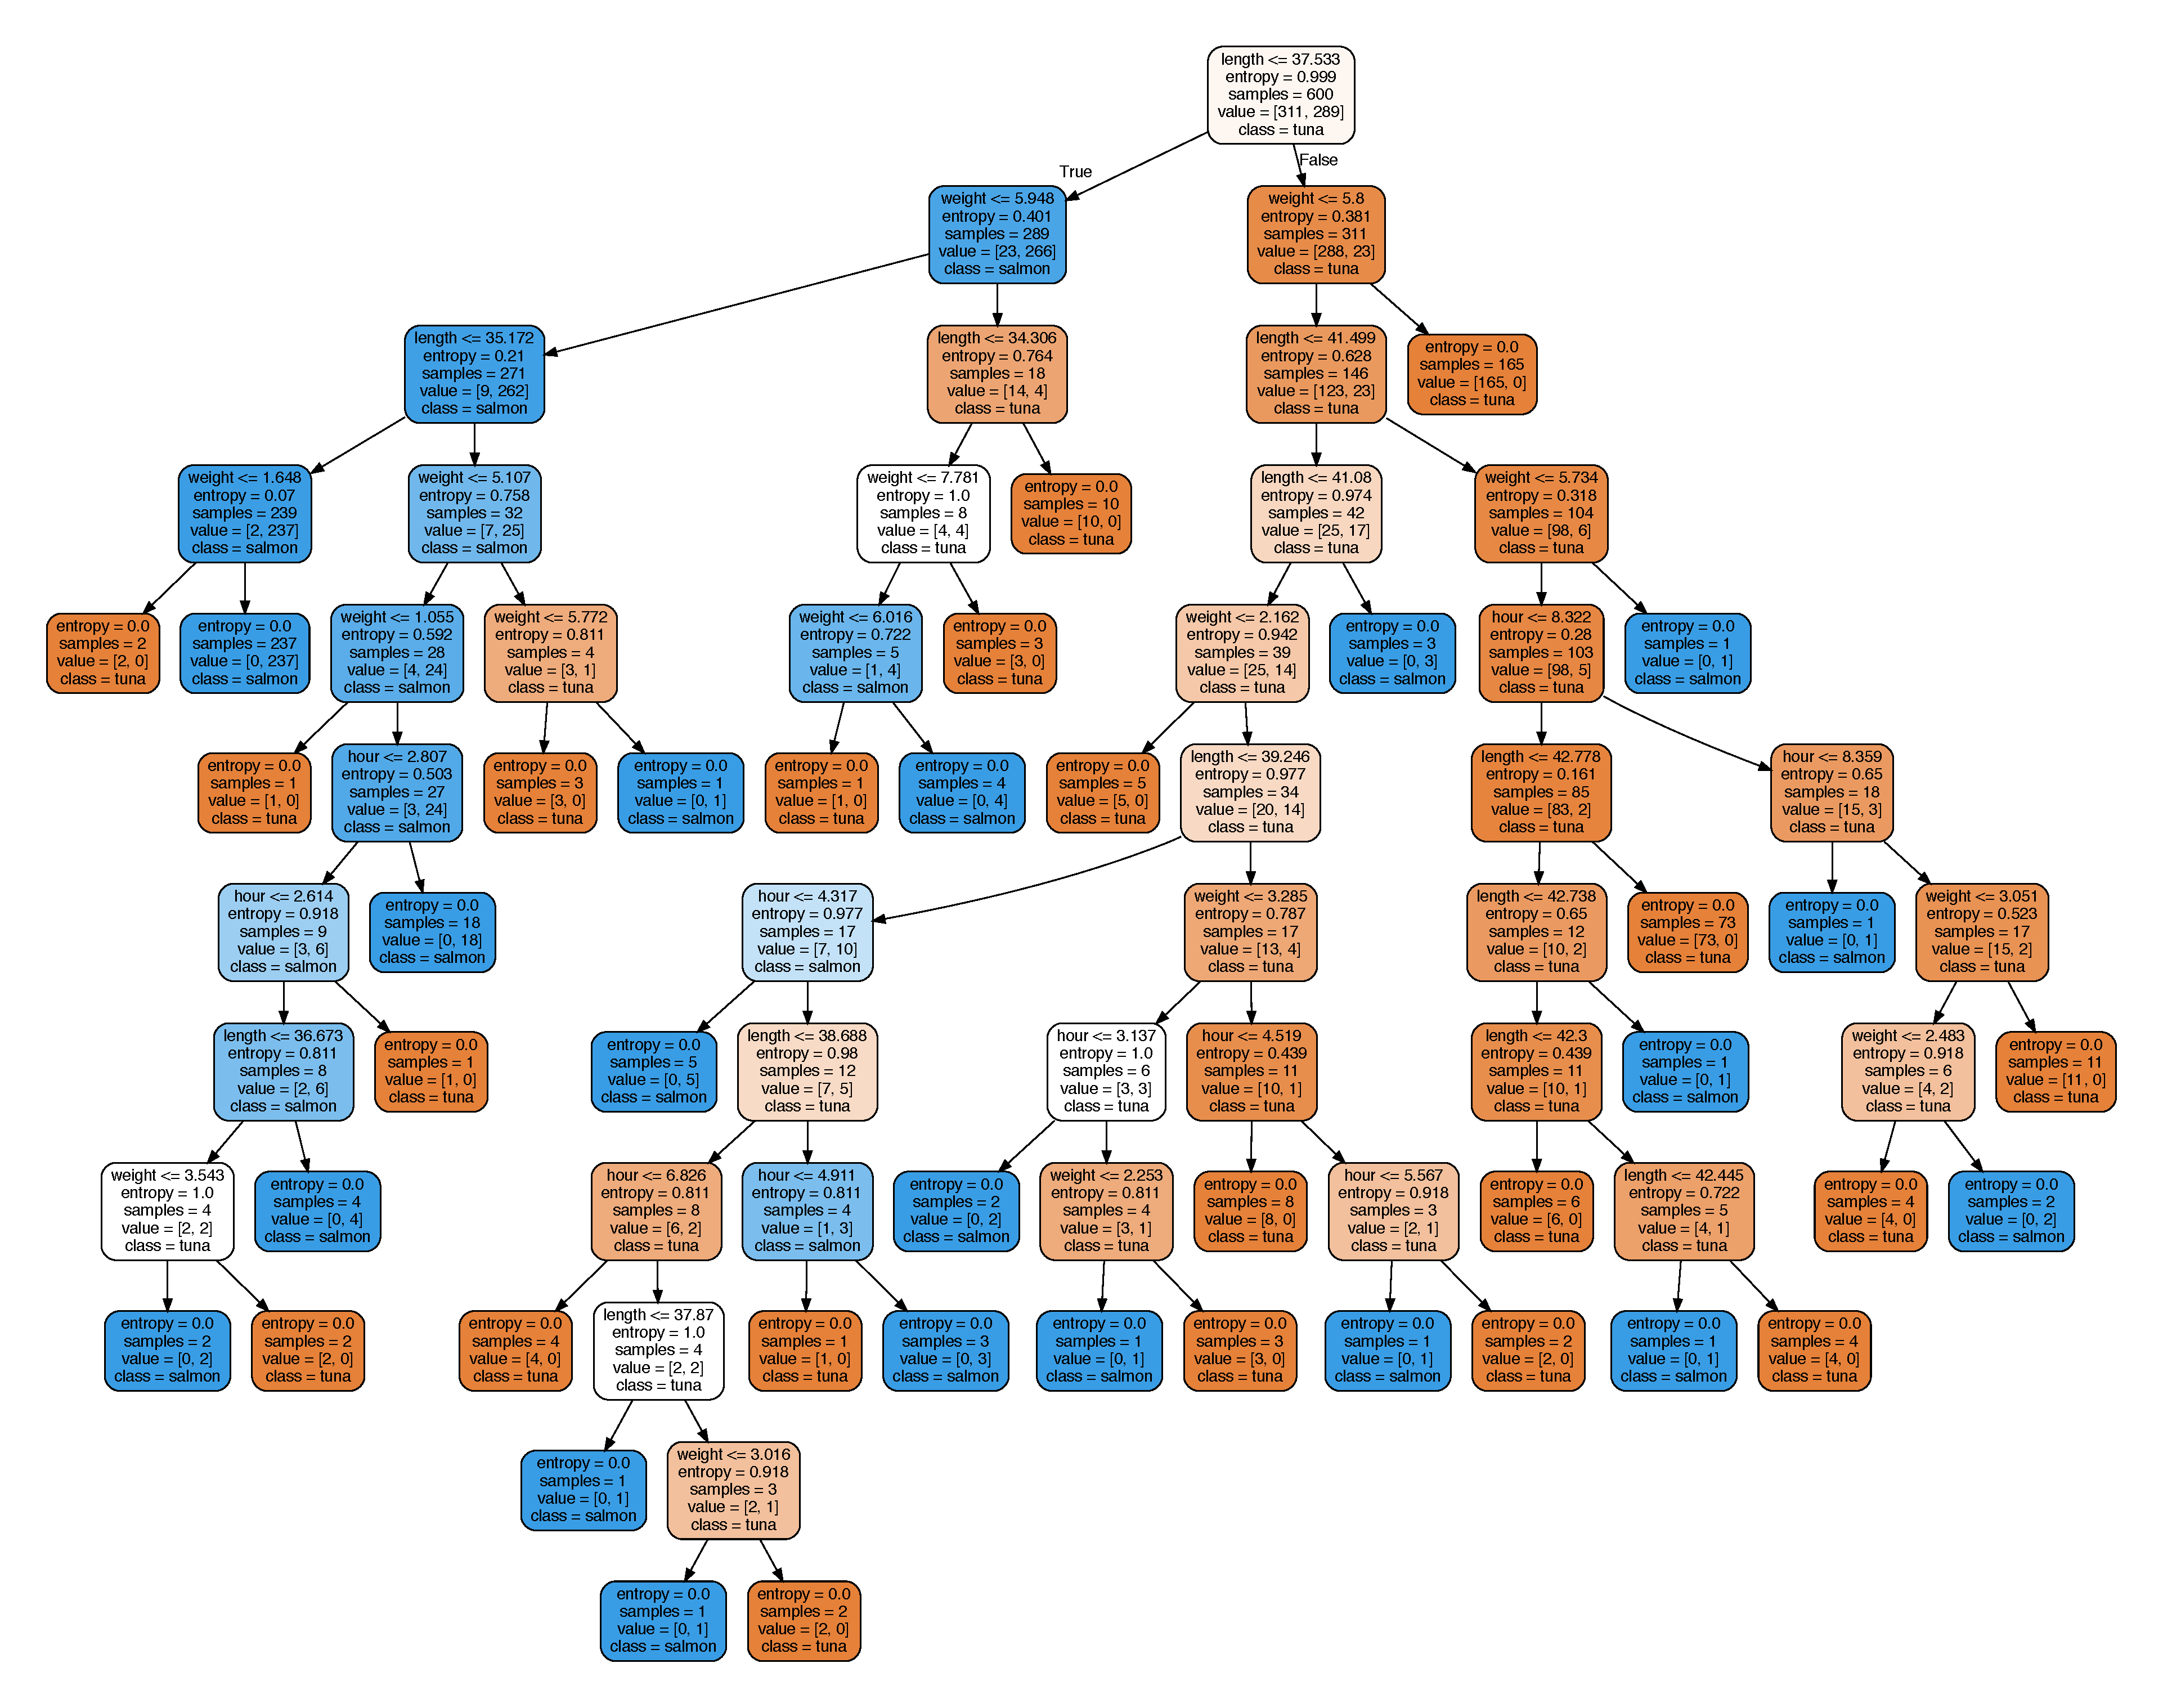
\includegraphics[width=0.7\linewidth]{fish_max_depth_12}
       \label{fig:}
   \end{figure} 
\end{frame}

\begin{frame}{Simulation: fish dataset}
   \begin{figure}[htpb]
       \centering
       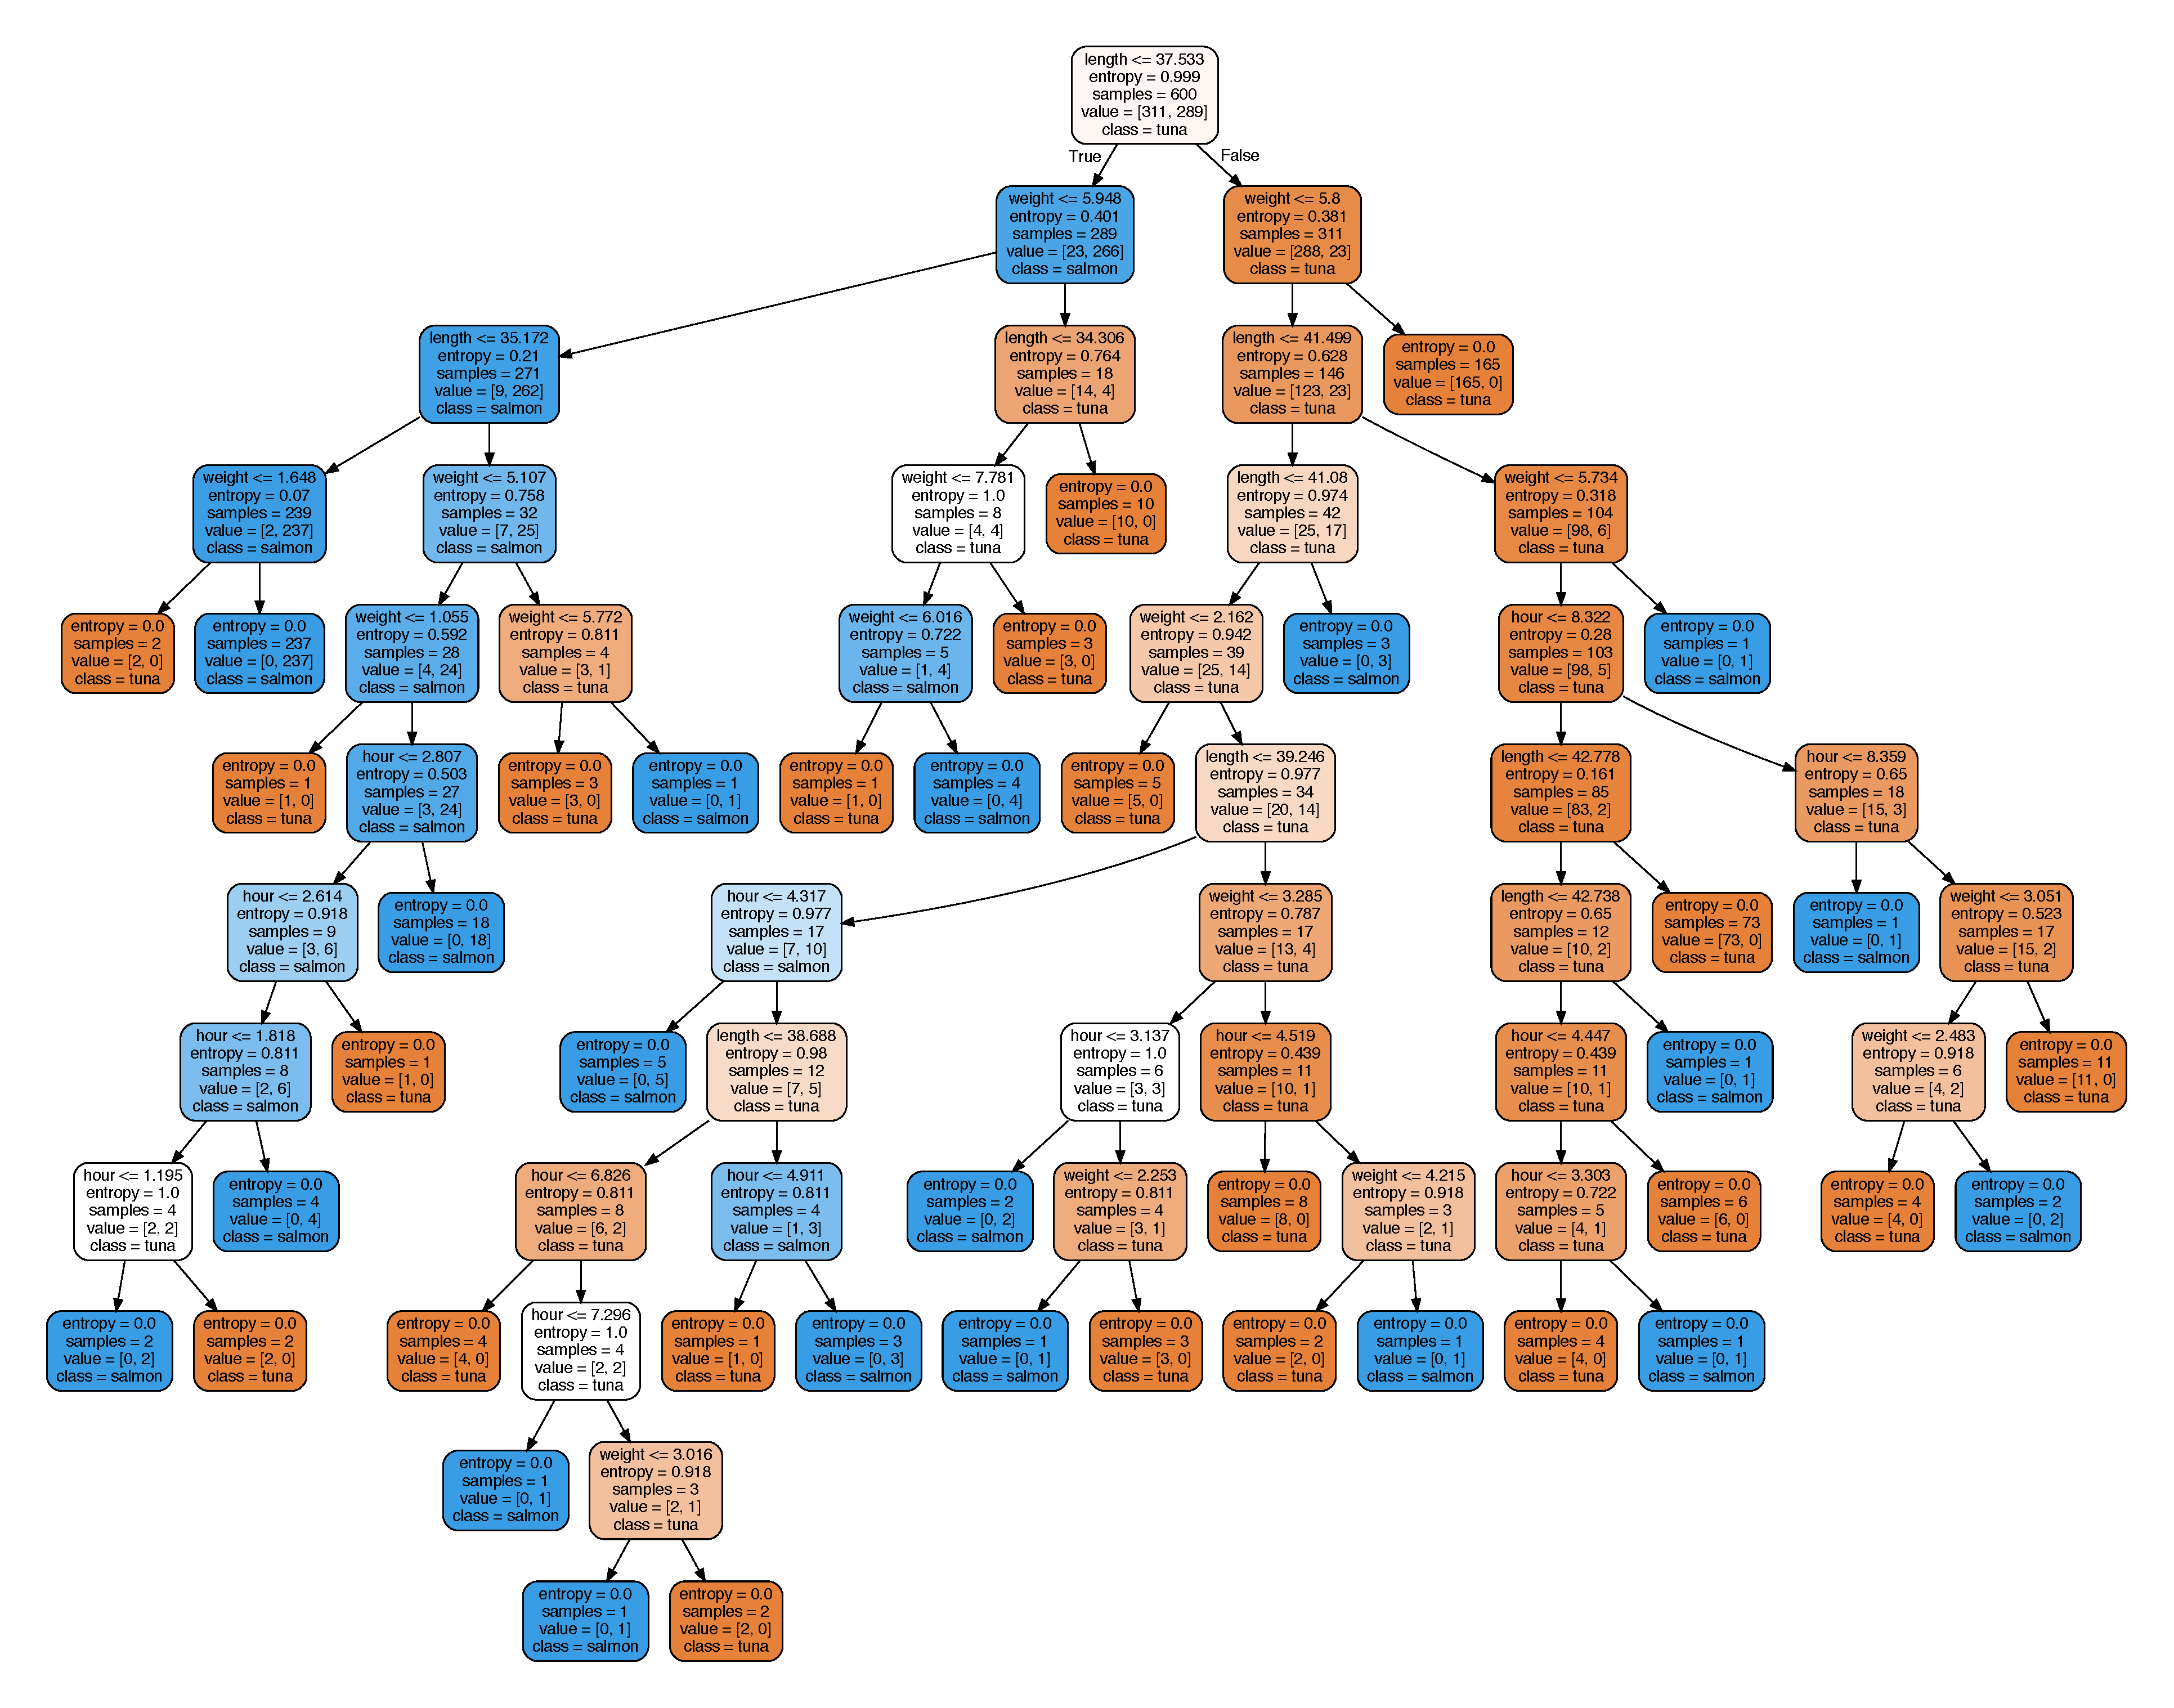
\includegraphics[width=0.7\linewidth]{fish_max_depth_34}
       \label{fig:}
   \end{figure} 
\end{frame}

\begin{frame}{Overfitting: Iris dataset, max depth=34}
    \begin{figure}[htpb]
        \centering
        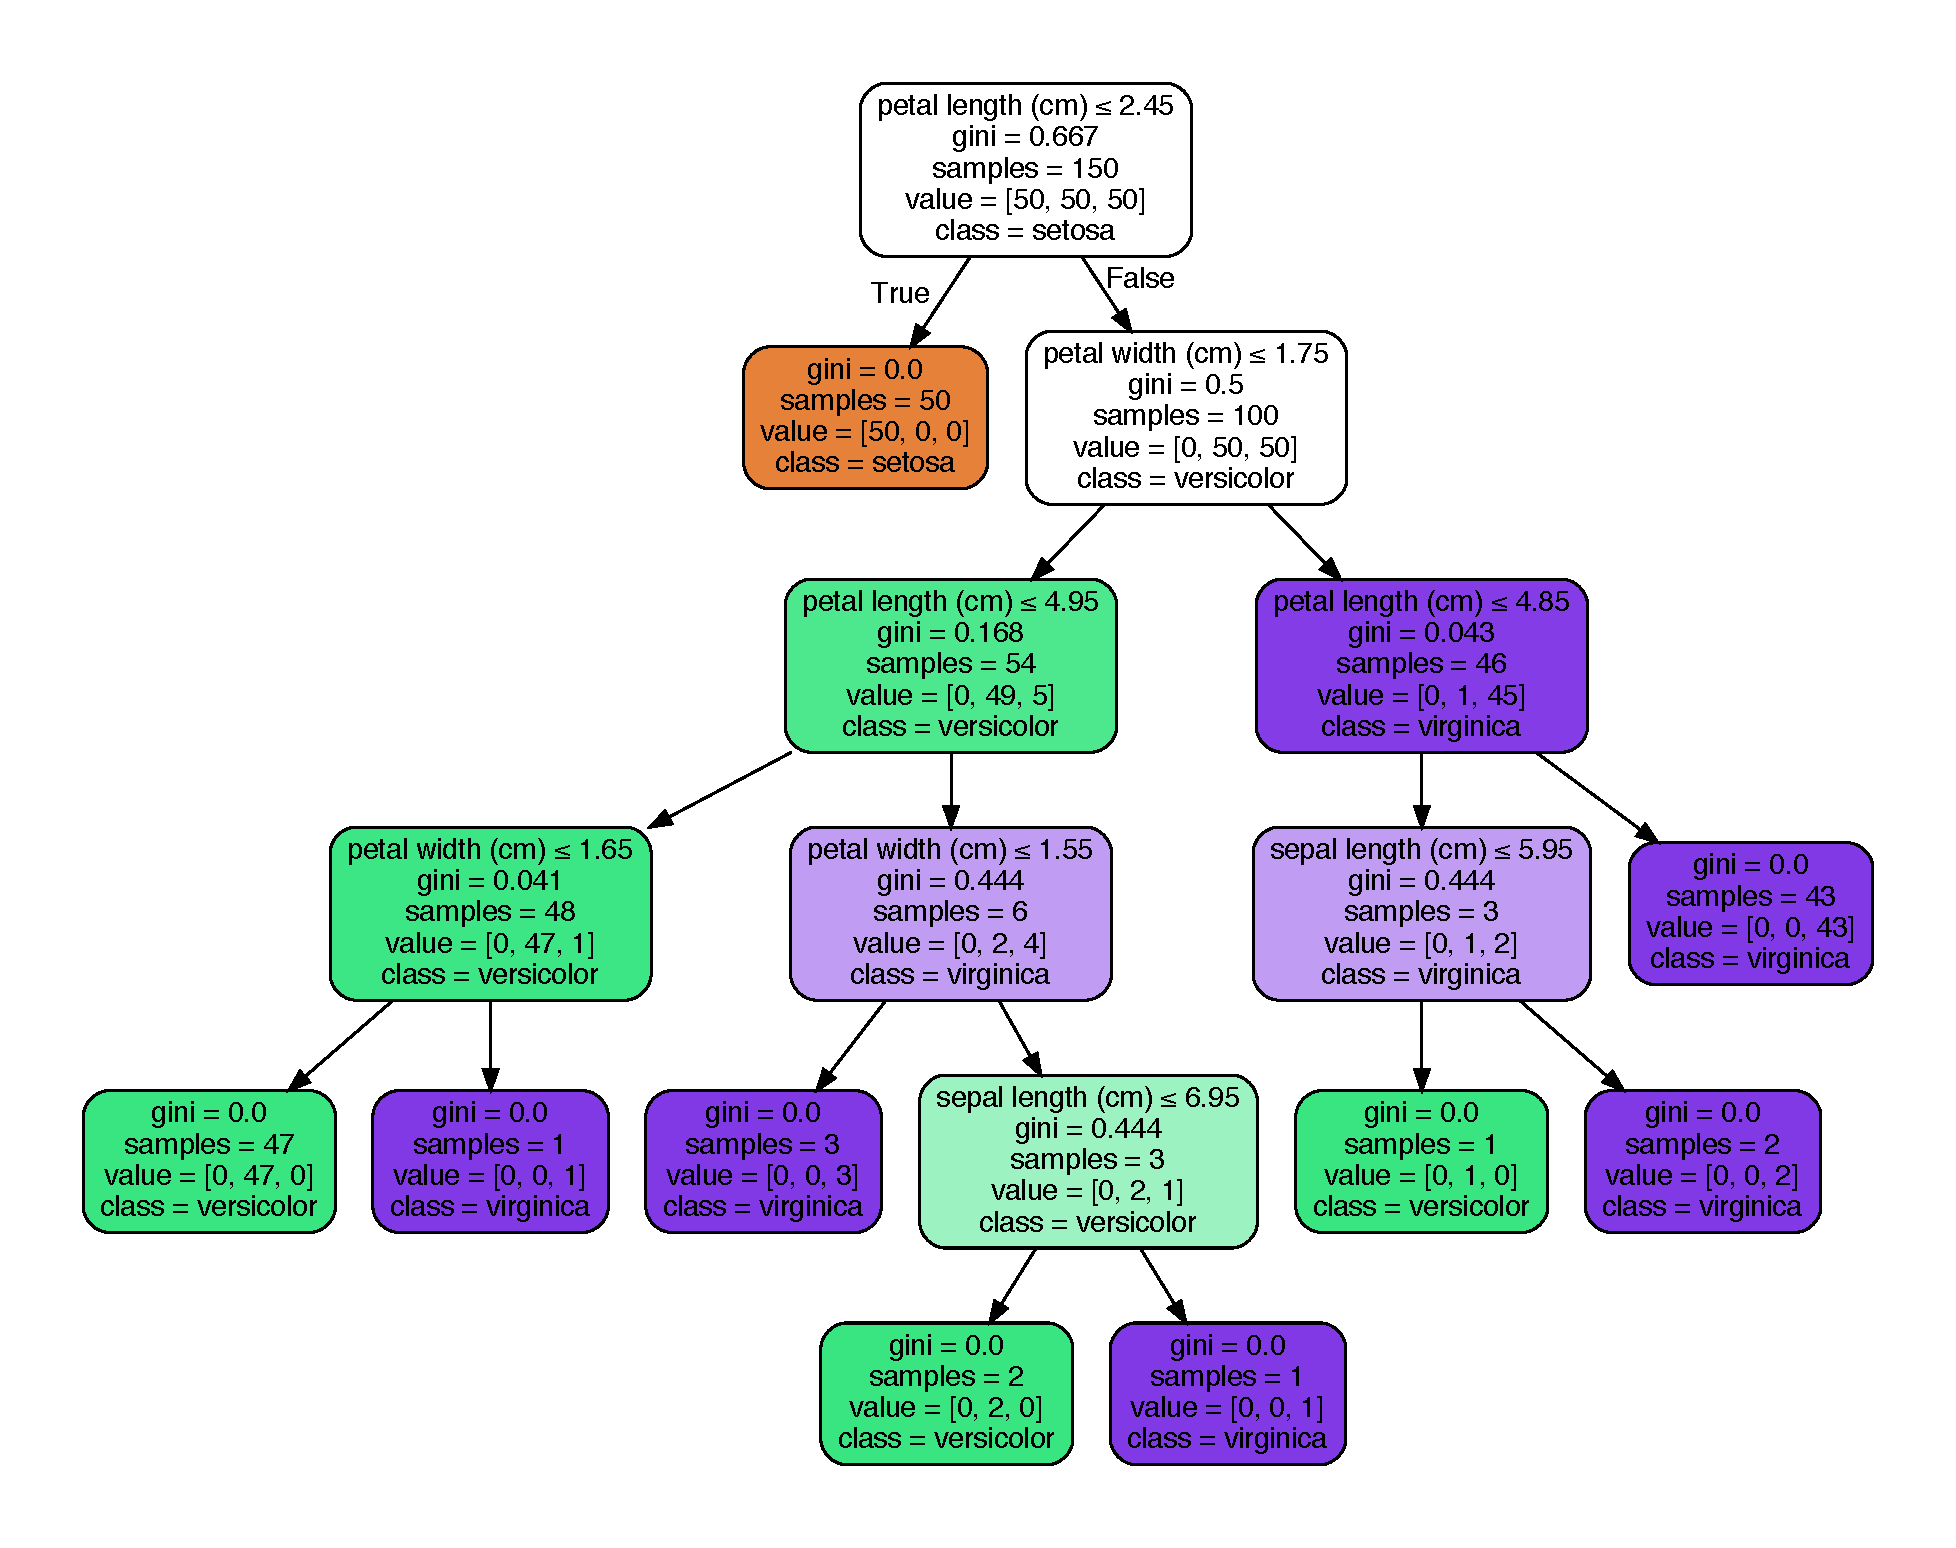
\includegraphics[width=0.8\linewidth]{tree_iris_overfit}
        \caption{Overfitting on the iris dataset.}
        \label{fig:tree_iris_overfit}
    \end{figure}
\end{frame}

\begin{frame}{Avoiding overfitting: Iris dataset}
    \exercice{}

    Avoid overfitting by choosing a pruning method on the iris dataset (\textbf{day\textunderscore 5/1\textunderscore cart/tree\textunderscore iris.py})
    \begin{figure}[htpb]
        \centering
        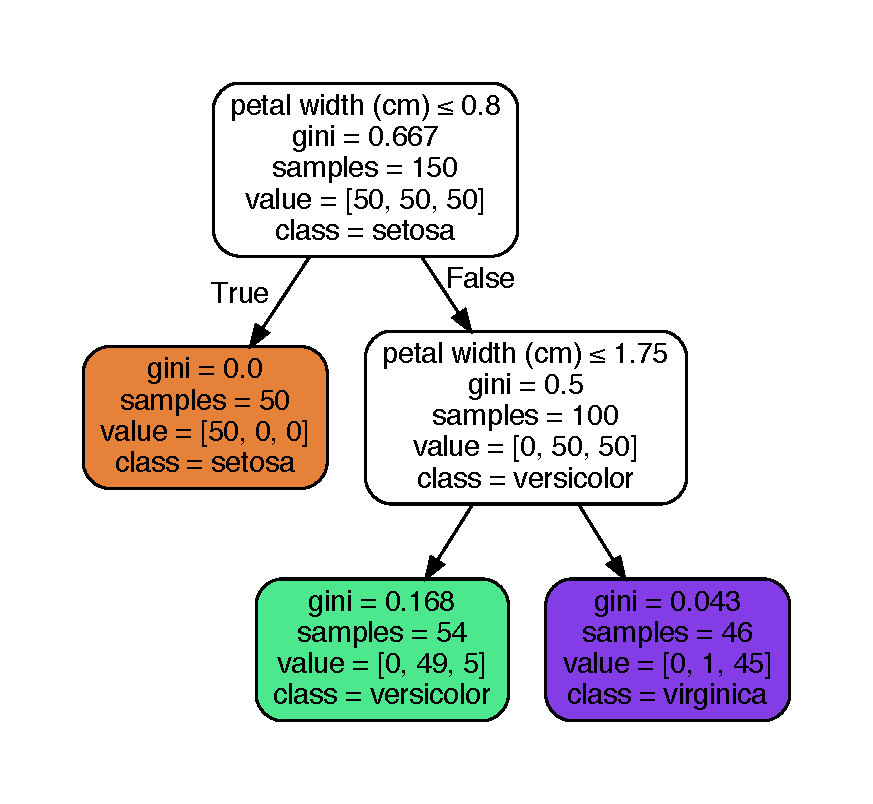
\includegraphics[width=0.4\linewidth]{tree_iris}
        \caption{Avoid overfitting with pre-pruning.}
        \label{fig:tree_iris_overfit}
    \end{figure}
\end{frame}

\begin{frame}{Post-pruning}

    It is also possible to prune after the construction of a large tree.
    
\end{frame}

\subsubsection{Remarks on decision trees}%
\label{ssub:}

\begin{frame}{Remarks on decision trees I}

    \begin{itemize}
        \item Decision trees do not require hypotheses on the distribution of the features.
	\item \textbf{Feature selection} (determinine which features matter for the quantity to predict) is integrated in the algorithm, so they might be relevant in a situation with many features (variables explicatives)
	\item Decision trees allow a straightforward \textbf{{interpretation}} of the model.
    \end{itemize}
    
\end{frame}


\begin{frame}{Remarks on decision trees II}
    \begin{itemize}
        \item Decision trees are greedy: they might find a local minimum
	\item they are hierarchical: a bad choice in a segmentation at the top of the tree propagates in the whole tree
	\item Hence their instability and sensibility to the choice of the training set.
    \end{itemize}
\end{frame}



\section{Ensemble learning}%
\frame{\tableofcontents[currentsection]}
\label{sec:ensemble_learning}

\begin{frame}{Ensemble learning}
    \begin{itemize}
	\item \textit{{Bagging}}  and \textit{{boosting}} are methods that combine estimators (in parallel or sequentially)
	\item they are often applied to decision trees
	\item they reach state-of-the-art performance in several supervised learning tasks \cite{Fernandez-Delgado2014}  (pdf in \textbf{documents/trees/} at the root of the repo)
	\item they are an active area of research (both theoretically and for practical applications).
    \end{itemize}

    \url{https://scikit-learn.org/stable/modules/ensemble.html} 
\end{frame}

\subsection{Bagging}%
\label{sub:bagging}


\begin{frame}{Aggregating}
    \begin{itemize}
        \item usual setup: input space $ \mathcal{X} $, output space $ \mathcal{Y} $.
	\item we note $z_b$ a dataset sampled from the unknown distribution $
        \rho$. If we sample $b$ different datasets, $b\in [1, B]$, 
	    \begin{equation}
		z_b = \{(x_{1b}, y_{1b}), \dots (x_{nb}, y_{nb})\}
	    \end{equation}
	\item we note $ \hat{f_{z_b}}$ the estimator obtained after learning with $ z_b$.
    \end{itemize}
\end{frame}

\begin{frame}{Aggregating: reducing the variance of the final estimator}
    \begin{itemize}
	\item we note $z_b$ a dataset sampled from the unknown distribution $ \rho$. If we sample $b$ different dataset, $b\in [1, B]$, 
	    \begin{equation}
		z_b = \{(x_{1b}, y_{1b}), \dots (x_{nb}, y_{nb})\}
	    \end{equation}
	\item we note $ \hat{f_{z_b}}$ the estimator obtained after learning with $ z_b$.
    \end{itemize}
    \textbf{{Aggregating}} consists in using as an estimator:
    \begin{itemize}
	\item for regression (usual averaging)
	    \begin{equation}
		\hat{f_B} = \frac{1}{B} \sum^{B}_{b=1} \hat{f_{z_b}}
	    \end{equation}
	\item for classification (majority in the vote)
	    \begin{equation}
		\hat{f_B}(x) = \argmax_{j} | \{ b, \hat{f_{z_b}}(x)=j \}|
	    \end{equation}
    \end{itemize}
\end{frame}

\begin{frame}{Bootstrapping and bagging}
    \begin{itemize}
    	\item If $B$ is large, it is not possible to sample $B$ independent datasets with $n$ samples, from a finite dataset.

    \textbf{{Bootstrapping}} consists in sampling $B$ times a sample dataset with $n$ elements \textbf{{with replacement}}.
	\item \textbf{{Bagging}} is the combination of bootstrapping and aggregating.
    \end{itemize}
    
\end{frame}

\begin{frame}{Out-of-bag error}
    
    For an observation $(x_i, y_i)$, the \textbf{{out-of-bag error}}  is the mean error on this observation among the estimators that were trained on a bootstrap dataset \textbf{{not}} containing it.

    It is the "bootstrapping version" of the test error.
\end{frame}


\begin{frame}{Trees and bagging}

    Bagging is most often used with decision trees. Several strategies are possible in order to build the base estimators $ \hat{f_{z_b}}$ and to prune them.
    \begin{itemize}
	\item pre-pruning by enforcing a minimal number of samples per leaf node (e.g. $5$): good tradeoff between computation speed and quality of the prediction. The goal is to reduce high variance of the base estimators by averaging.
	\item pre-pruning by enforcing a maximal tree depth or maximal number of leaves.
    \end{itemize}
\end{frame}

\begin{frame}{Simulation}
    \begin{figure}[htpb]
        \centering
        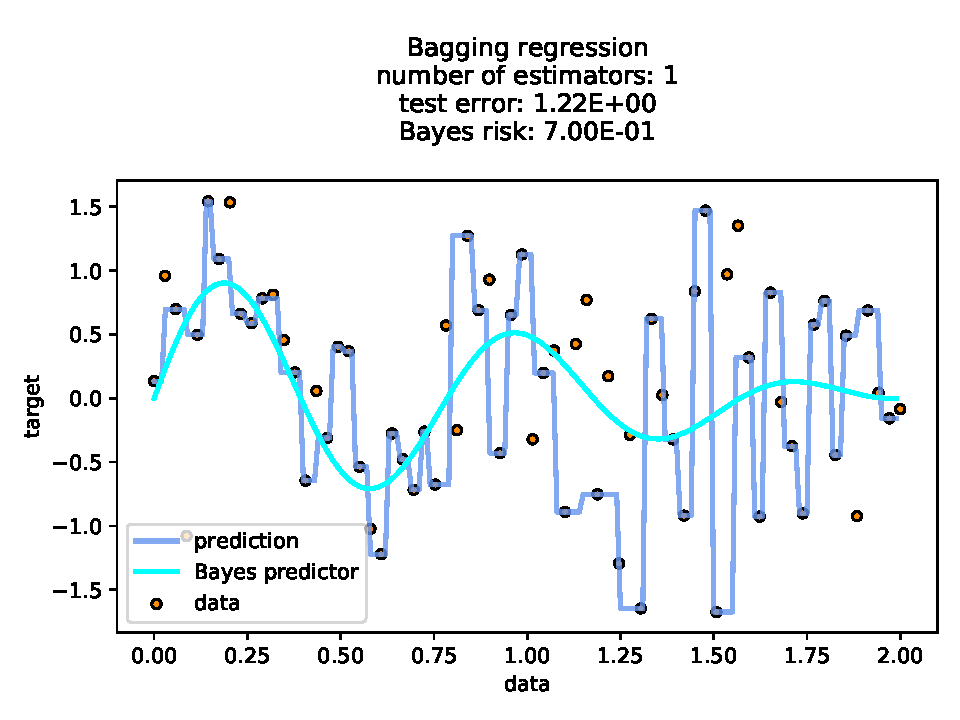
\includegraphics[width=0.8\linewidth]{bagging/Bagging_regression_nest_1}
        \label{fig:bagging/Bagging regression_nest_1}
    \end{figure}
\end{frame}


\begin{frame}{Simulation}
    \begin{figure}[htpb]
        \centering
        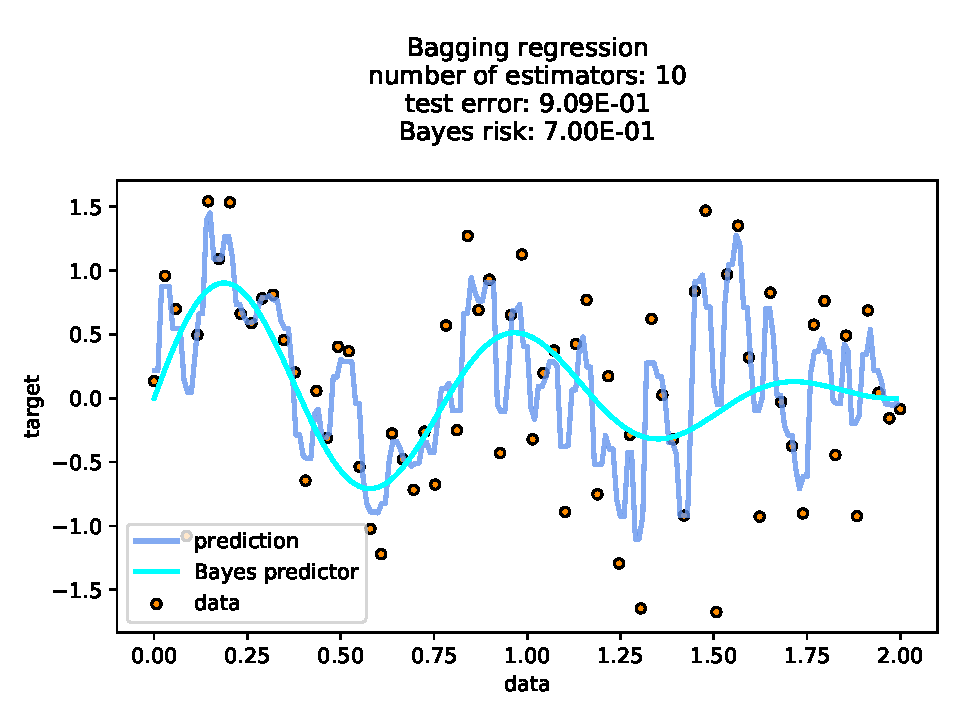
\includegraphics[width=0.8\linewidth]{bagging/Bagging_regression_nest_10}
        \label{fig:bagging/Bagging regression_nest_1}
    \end{figure}
\end{frame}


\begin{frame}{Simulation}
    \begin{figure}[htpb]
        \centering
        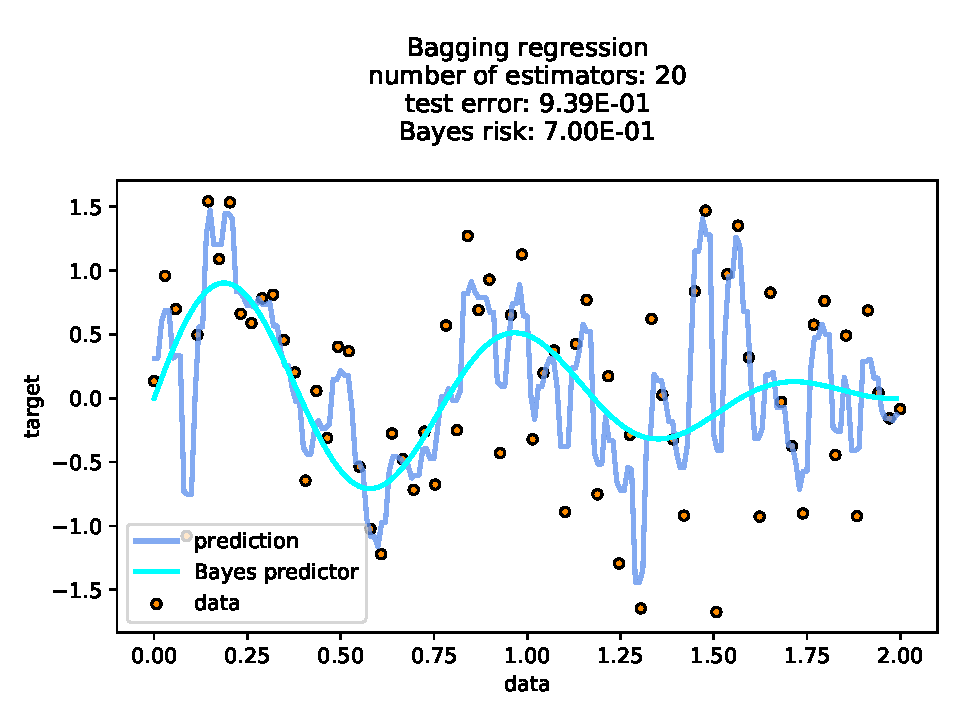
\includegraphics[width=0.8\linewidth]{bagging/Bagging_regression_nest_20}
        \label{fig:bagging/Bagging regression_nest_1}
    \end{figure}
\end{frame}


\begin{frame}{Simulation}
    \begin{figure}[htpb]
        \centering
        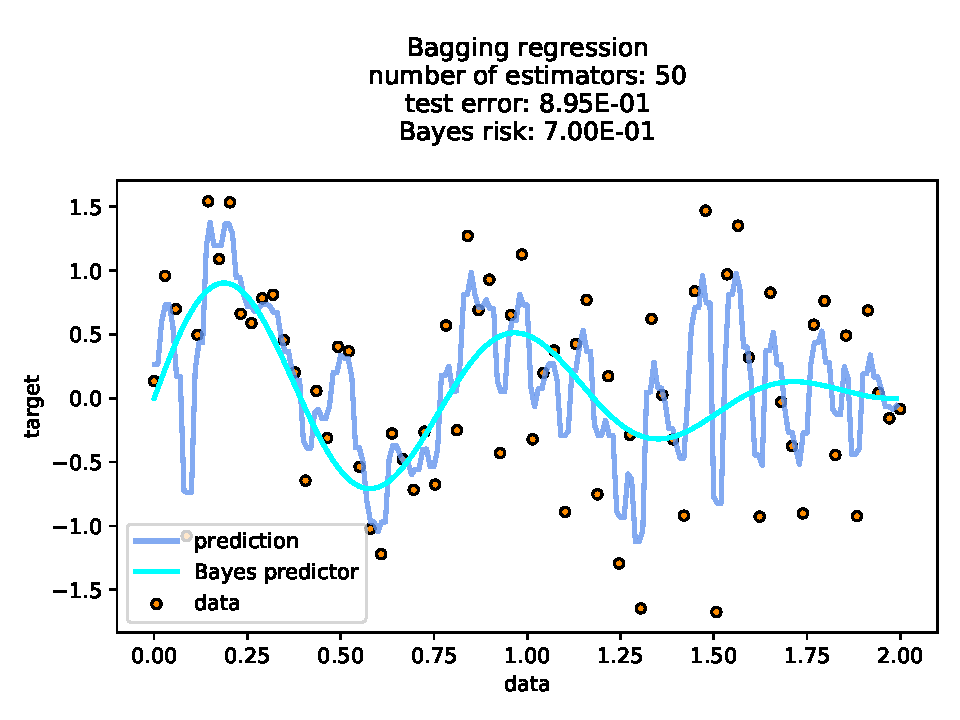
\includegraphics[width=0.8\linewidth]{bagging/Bagging_regression_nest_50}
        \label{fig:bagging/Bagging regression_nest_1}
    \end{figure}
\end{frame}


\begin{frame}{Simulation}
    \begin{figure}[htpb]
        \centering
        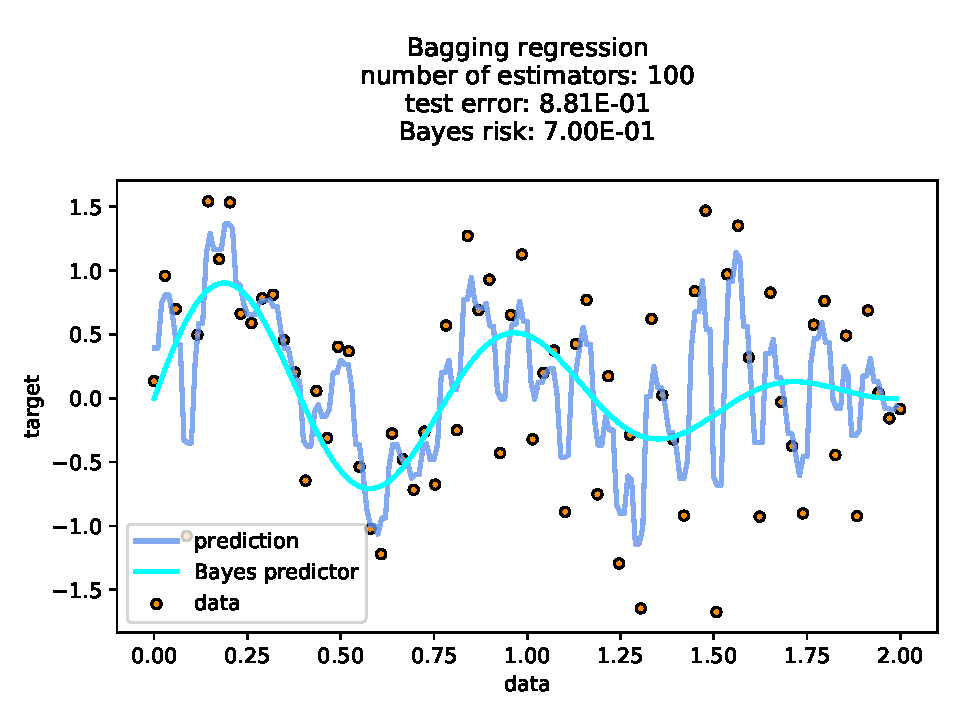
\includegraphics[width=0.8\linewidth]{bagging/Bagging_regression_nest_100}
        \label{fig:bagging/Bagging regression_nest_1}
    \end{figure}
\end{frame}

\begin{frame}{Individual estimators}
    \begin{figure}[htpb]
        \centering
        
\includegraphics[width=1\linewidth]{bagging/estimator_0}
        \caption{Estimator used in the averaging}
        \label{fig:bagging/estimator_0}
    \end{figure}
\end{frame}

\begin{frame}{Individual estimators}
    \begin{figure}[htpb]
        \centering
        
\includegraphics[width=1\linewidth]{bagging/estimator_1}
        \caption{Other estimator used in the averaging}
        \label{fig:estimator_0}
    \end{figure}
\end{frame}


\begin{frame}{Possible issues}
    \begin{itemize}
	\item number of trees to compute ($B$) in order to have a stable out-of-bag error.
	\item need for storing all the base estimators
	\item the final estimator is a \textit{{black-box}} model.
    \end{itemize}
\end{frame}

\subsection{Random forest}%
\label{sub:random_forests}

\begin{frame}{Random forest}
    \begin{itemize}
        \item Random forest \cite{Breiman2001} is a bagging method with binary CART estimators, with additional randomness added to the choice of segmentation variables.
	\item the goal is to increase the \textbf{{independence}} between the base trees.
	\item although the theoretical properties of random forest are not yet fully understood, it is an important benchmark in supervised learning (but for instance not when the problem can be solved in a linear way).
    \end{itemize}
\end{frame}

\begin{frame}{Random forest II}
    \begin{itemize}
	\item With random forests, it is possible to use a more brutal pruning (for instance using only trees of depth $2$)
	\item To tune $m$, heuristics are used. Common ones include:
	    \begin{itemize}
		\item $m = \sqrt{d} $ for classification ($d$ is the number of features)
		\item $m = d/3$ for regression
		\item cross validation.
	    \end{itemize}
    \end{itemize}
\end{frame}

\begin{frame}{Example in 1D (1 feature, hence not really illustrative of random forest !)}
    \begin{figure}[htpb]
        \centering
        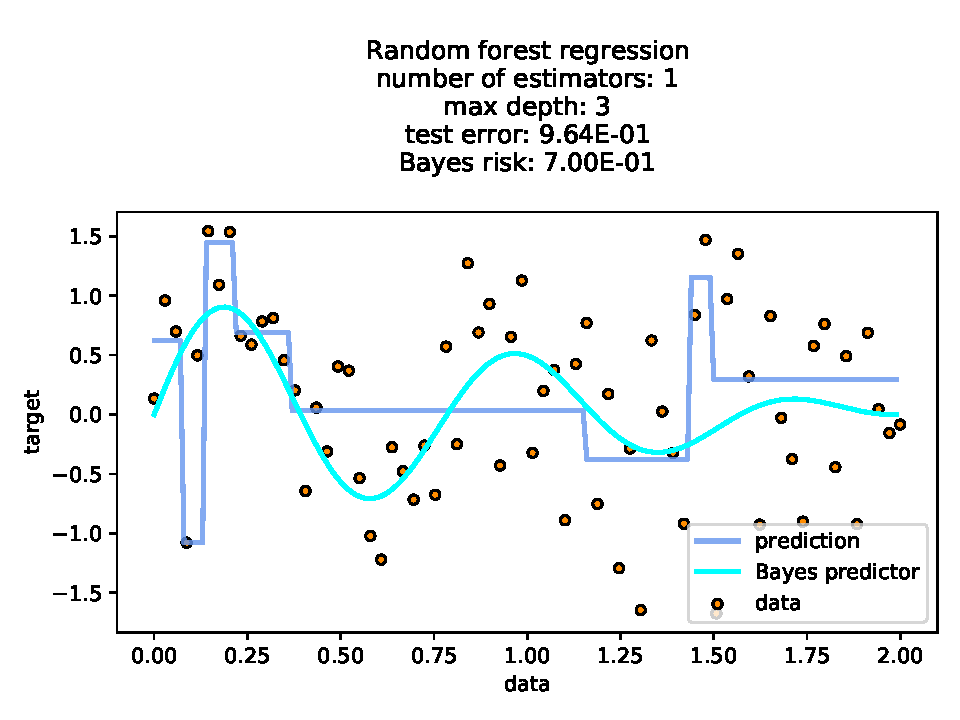
\includegraphics[width=0.8\linewidth]{forest/Random_forest_regression_nest_1_d_3}
        \label{fig:forest/Random_forest_regression_nest_1_d_3}
    \end{figure}
\end{frame}


\begin{frame}{Example in 1D}
    \begin{figure}[htpb]
        \centering
        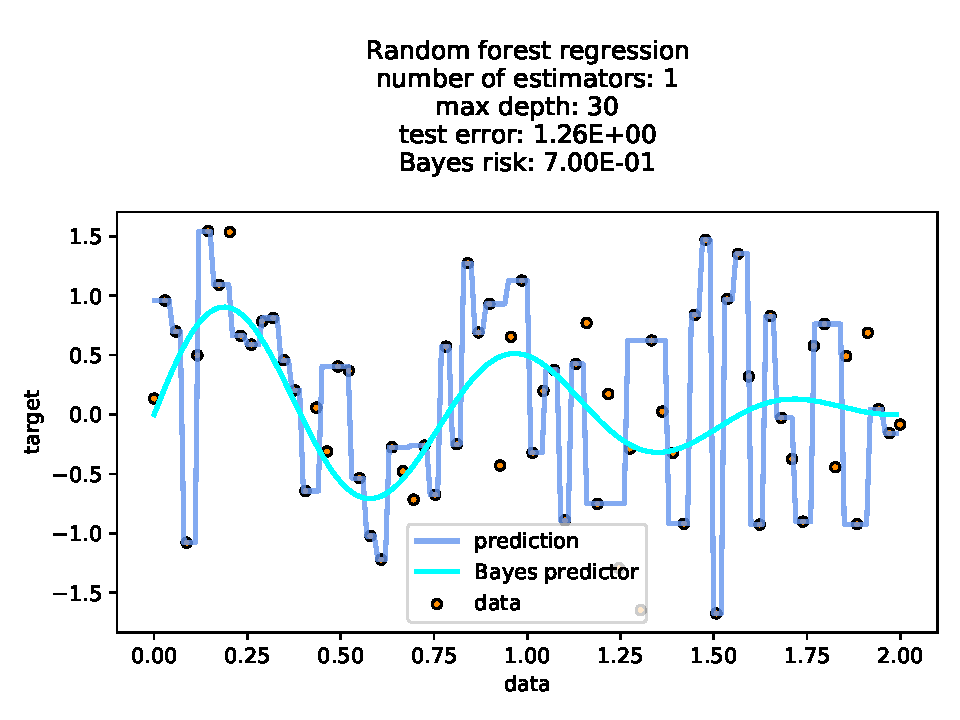
\includegraphics[width=0.8\linewidth]{forest/Random_forest_regression_nest_1_d_30}
        \label{fig:forest/Random_forest_regression_nest_1_d_3}
    \end{figure}
\end{frame}


\begin{frame}{Example in 1D}
    \begin{figure}[htpb]
        \centering
        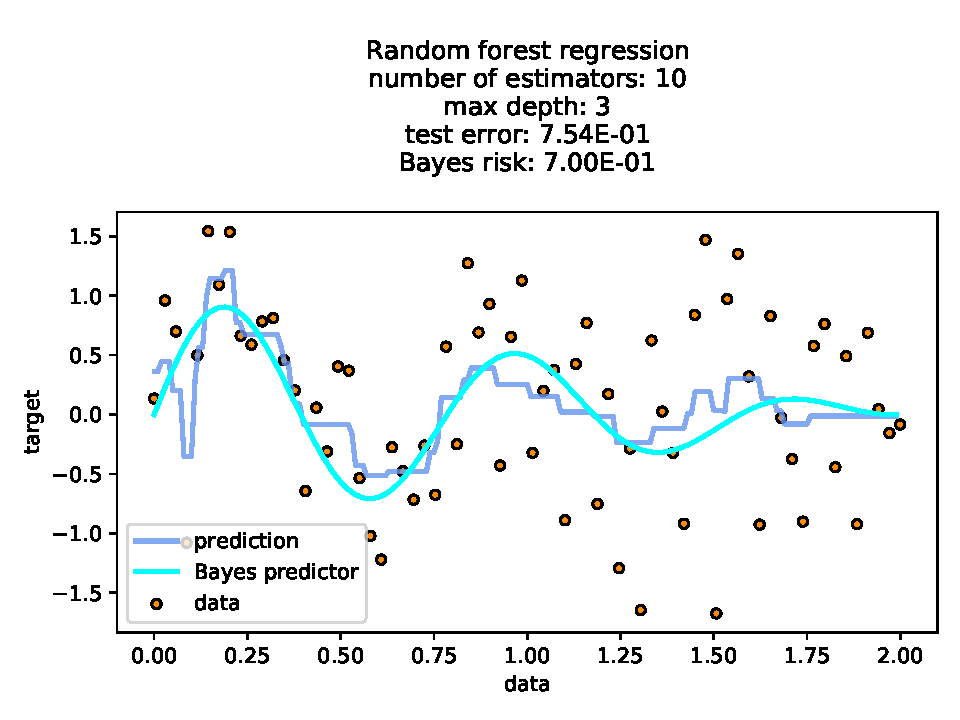
\includegraphics[width=0.8\linewidth]{forest/Random_forest_regression_nest_10_d_3}
        \label{fig:forest/Random_forest_regression_nest_1_d_3}
    \end{figure}
\end{frame}


\begin{frame}{Example in 1D}
    \begin{figure}[htpb]
        \centering
        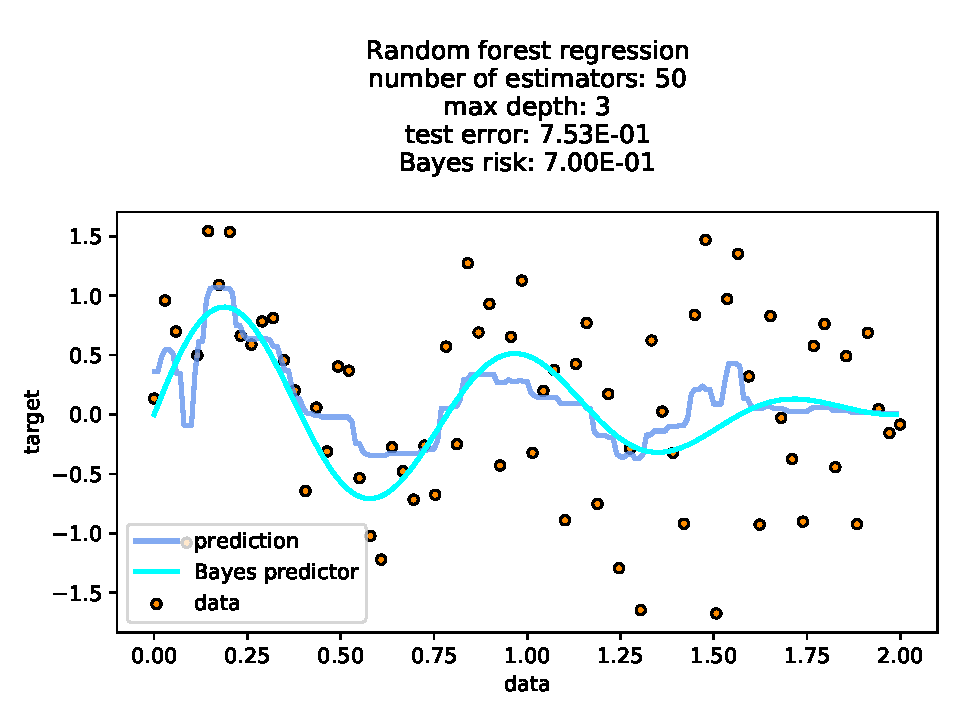
\includegraphics[width=0.8\linewidth]{forest/Random_forest_regression_nest_50_d_3}
        \label{fig:forest/Random_forest_regression_nest_1_d_3}
    \end{figure}
\end{frame}


\begin{frame}{Example in 1D}
    \begin{figure}[htpb]
        \centering
        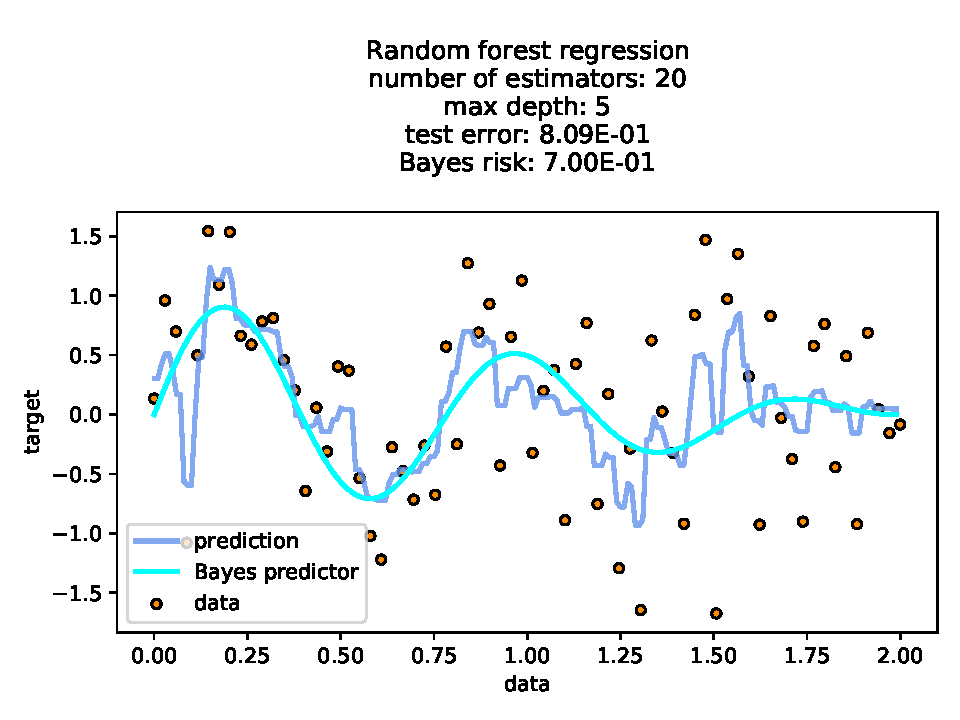
\includegraphics[width=0.8\linewidth]{forest/Random_forest_regression_nest_20_d_5}
        \label{fig:forest/Random_forest_regression_nest_1_d_3}
    \end{figure}
\end{frame}

\begin{frame}{Estimators}
    \begin{figure}[htpb]
        \centering
        
\includegraphics[width=0.8\linewidth]{forest/estimator_0}
        \label{fig:}
    \end{figure}
    
\end{frame}

\begin{frame}{Mean decrease accuracy}

    Although the final estimator is hard to interpret, we can still study the \textbf{importance of features} for the prediction.

    We consider a feature $j$. For a given tree $b$
   \begin{itemize}
       \item compute the out-of-bag error
	\item shuffle the values of $j$ in the out-of-bag sample.
	\item compute the new out-of-bag error
	\item store the decrease in prediction quality, $D_j^b$.
   \end{itemize} 

    Average the $D_j^b$ over all the estimators $b$ in order to measure the importance of feature $j$.

\end{frame}

\begin{frame}{Other hyperparameters}
    Many hyperparameters are involved for ensemble learning.
    \begin{itemize}
	\item \textbf{{subsampling}}: sampling bootstrap datasets of size $s<n$. Smaller variance because of more independence between the trees, but higher bias.
	\item number of bins in each variable (for instance, impose a maximum number of bins).
    \end{itemize}
\end{frame}


\begin{frame}{See also}

    \begin{itemize}
	\item boosting
	\item gradient tree boosting
        \item XGBoost: variant of gradient boosting, very efficient on several
            benchmarks \cite{Chen2016} 
	\item can exploit parallelization
	 \item \url{https://xgboost.readthedocs.io/en/latest/parameter.html} 
        \item \url{https://github.com/dmlc/xgboost} 
        \item See also: Catboost \url{https://catboost.ai/} 
    \end{itemize}
\end{frame}

\begin{frame}[allowframebreaks]
\frametitle{References}
\bibliographystyle{apalike}
\bibliography{epita.bib} 
\end{frame}


\end{document} 
